%%
%%
\begin{flushleft}
    \setlength{\parskip}{10pt}

    {\fontsize{12}{0} \bf 4. 實驗結果}
\end{flushleft}
%

%   AlexNet
\begin{abstract}
    \noindent\textbf{A. AlexNet}\\
    原始資料訓練特點
    \begin{enumerate}
        \item Batch Size 值較小時,Epoch的增加Loss無明顯下降,表現差不多。
        \item Batch Size 值較大時,Epoch的增加Training Loss明顯下降。
    \end{enumerate}
    加入GAN的訓練結果
    \begin{enumerate}
        \item Epoch值較小時,Loss表現與原始資料差不多。
        \item Epoch值較大時,Loss表現能看出比原始資料好一點。
    \end{enumerate}
\end{abstract}
%
\begin{figure}[H]
    \centering
    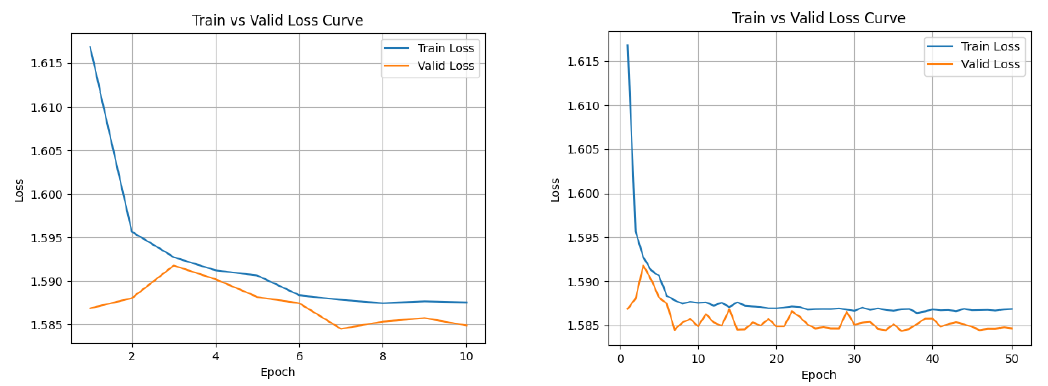
\includegraphics[width=0.45\textwidth]{./img/AlexNet/b8_lr1e-3_loss.png}
    \caption{AlexNet B8 Lr1e-3 Loss曲線\protect\\(左:epoch10,右:epoch50)}
    \label{fig:AlexNet_b8_lr1e-3_loss_curve}
\end{figure}
\begin{figure}[H]
    \centering
    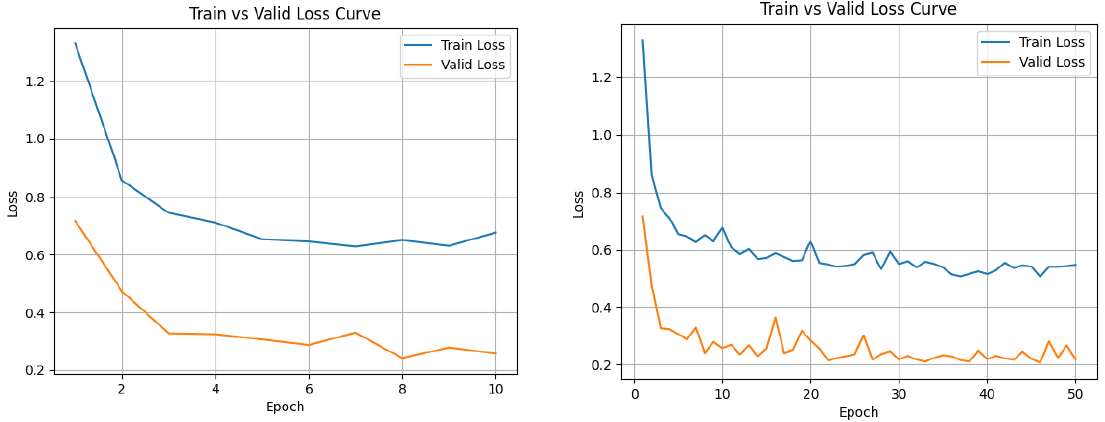
\includegraphics[width=0.45\textwidth]{./img/AlexNet/b32_lr1e-3_loss.png}
    \caption{AlexNet B32 Lr1e-3 Loss曲線\protect\\(左:epoch10,右:epoch50)}
    \label{fig:AlexNet_b32_lr1e-3_loss_curve}
\end{figure}
\begin{figure}[H]
    \centering
    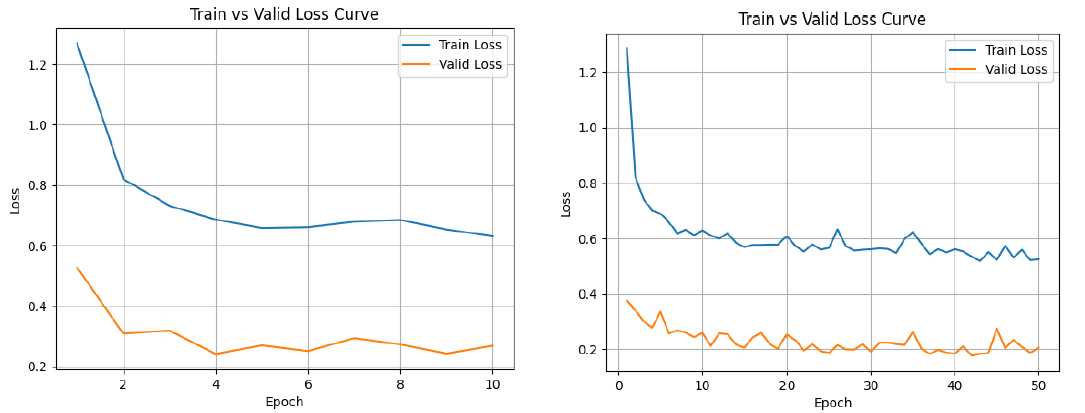
\includegraphics[width=0.45\textwidth]{./img/AlexNet/b32_lr1e-3_GAN_loss.png}
    \caption{AlexNet B32 Lr1e-3 GAN Loss曲線\protect\\(左:epoch10,右:epoch50)}
    \label{fig:AlexNet_b32_lr1e-3_GAN_loss_curve}
\end{figure}
%
\FloatBarrier

%   VGG
\begin{abstract}
    \noindent\textbf{B. VGG}\\
    \hspace*{2em}此模型在learning rate為2e-5時訓練成效最佳,而在learning rate為1e-3及1e-4時無法正確檢測各瑕疵。\\
    learning rate為1e-3及1e-4的訓練結果:
    \begin{enumerate}
        \item train loss與valid loss約會停留在1.58~1.595之間,如圖\ref{fig:VGG_P1}(learning rate = 1e-3,batch size = 8)、圖\ref{fig:VGG_P2}(learning rate = 1e-4,batch size = 8)。
        \item 兩者並無法正確檢測出瑕疵,由confusion matrix(圖\ref{fig:VGG_P3})可以看出,其檢測結果皆集中於good上。
        \item 增加了GAN生成的資料集後,其train loss與valid losss約會停留在1.65~1.665之間,如圖\ref{fig:VGG_P4}(learning rate = 1e-3,batch size = 8)、圖\ref{fig:VGG_P5}(learning rate = 1e-4,batch size = 8),
              且依然無法正確檢測出瑕疵,confusion matrix與可視化結果如圖\ref{fig:VGG_P6}、圖\ref{fig:VGG_P7}所示。
        \item 原資料集的Precision固定為0.0715,增加GAN生成圖片的資料集Precision固定為0.0662,Recall皆固定為0.1429。
    \end{enumerate}
    learning rate為2e-5的訓練結果:
    \begin{enumerate}
        \item train loss會收斂至0.01以下,valid loss收斂的位置,batch size為8時,會比32與64還小,但皆在0.01附近,如圖\ref{fig:VGG_P8}(batch size = 8)
        \item 資料集與增加GAN生成的資料集的準確率皆能達到97.5\%以上。
        \item 增加GAN生成圖片的資料集不一定會較準確,有時會比原資料集大,有時較小,但若將所有fold中的各個batch size的test accuracy加總做平均計算,
              會發現增加GAN生成圖片的資料集平均(98.267\%)會比原始資料集(98.483\%)低。此learning rate的confusion matrix與可視化結果如圖\ref{fig:VGG_P9}、圖\ref{fig:VGG_P10}所示。
        \item Precision與Recall皆能達到0.95以上。
    \end{enumerate}
    不同learning rate下表現懸殊的情況,推測原因有二:
    \begin{enumerate}
        \item 資料集的分布較不平均,good資料集的總數明顯比其他資料集大上許多,因此訓練的模型可能較無法分辨各種瑕疵,這也能解釋為何confusion maitrix上的辨識結果都會集中在good上。
        \item VGG模型訓練的learning rate不能太大,由設定的三個參數中可以得知,最小的2e-5表現明顯比1e-3、1e-4優異。
    \end{enumerate}
\end{abstract}
%
\begin{figure}[H]
    \centering
    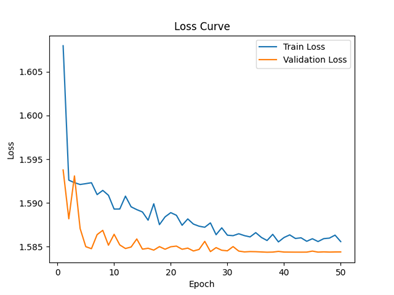
\includegraphics[width=0.45\textwidth]{./img/VGG/P1.png}
    \caption{VGG B8 Lr1e-3 Loss曲線}
    \label{fig:VGG_P1}
\end{figure}
\begin{figure}[H]
    \centering
    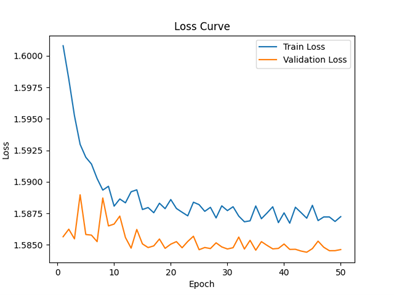
\includegraphics[width=0.45\textwidth]{./img/VGG/P2.png}
    \caption{VGG B8 Lr1e-4 Loss曲線}
    \label{fig:VGG_P2}
\end{figure}
\begin{figure}[H]
    \centering
    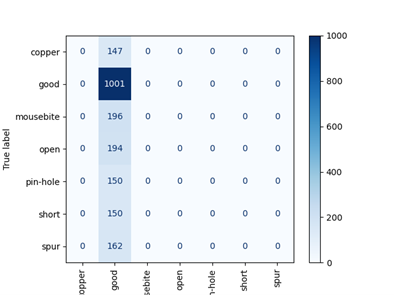
\includegraphics[width=0.45\textwidth]{./img/VGG/P3.png}
    \caption{VGG confusion matrix}
    \label{fig:VGG_P3}
\end{figure}
\begin{figure}[H]
    \centering
    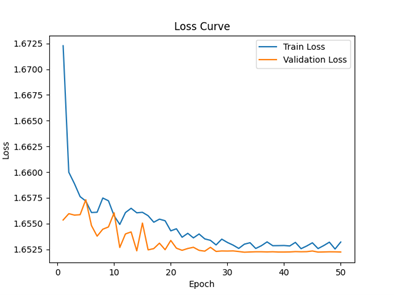
\includegraphics[width=0.45\textwidth]{./img/VGG/P4.png}
    \caption{VGG B8 Lr1e-3 GAN Loss曲線}
    \label{fig:VGG_P4}
\end{figure}
\begin{figure}[H]
    \centering
    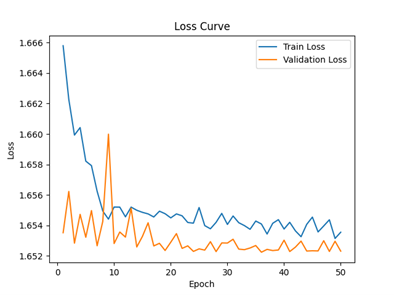
\includegraphics[width=0.45\textwidth]{./img/VGG/P5.png}
    \caption{VGG B8 Lr1e-4 GAN Loss曲線}
    \label{fig:VGG_P5}
\end{figure}
\begin{figure}[H]
    \centering
    \includegraphics[width=0.45\textwidth]{./img/VGG/P6.png}
    \caption{VGG GAN confusion matrix}
    \label{fig:VGG_P6}
\end{figure}
\begin{figure}[H]
    \centering
    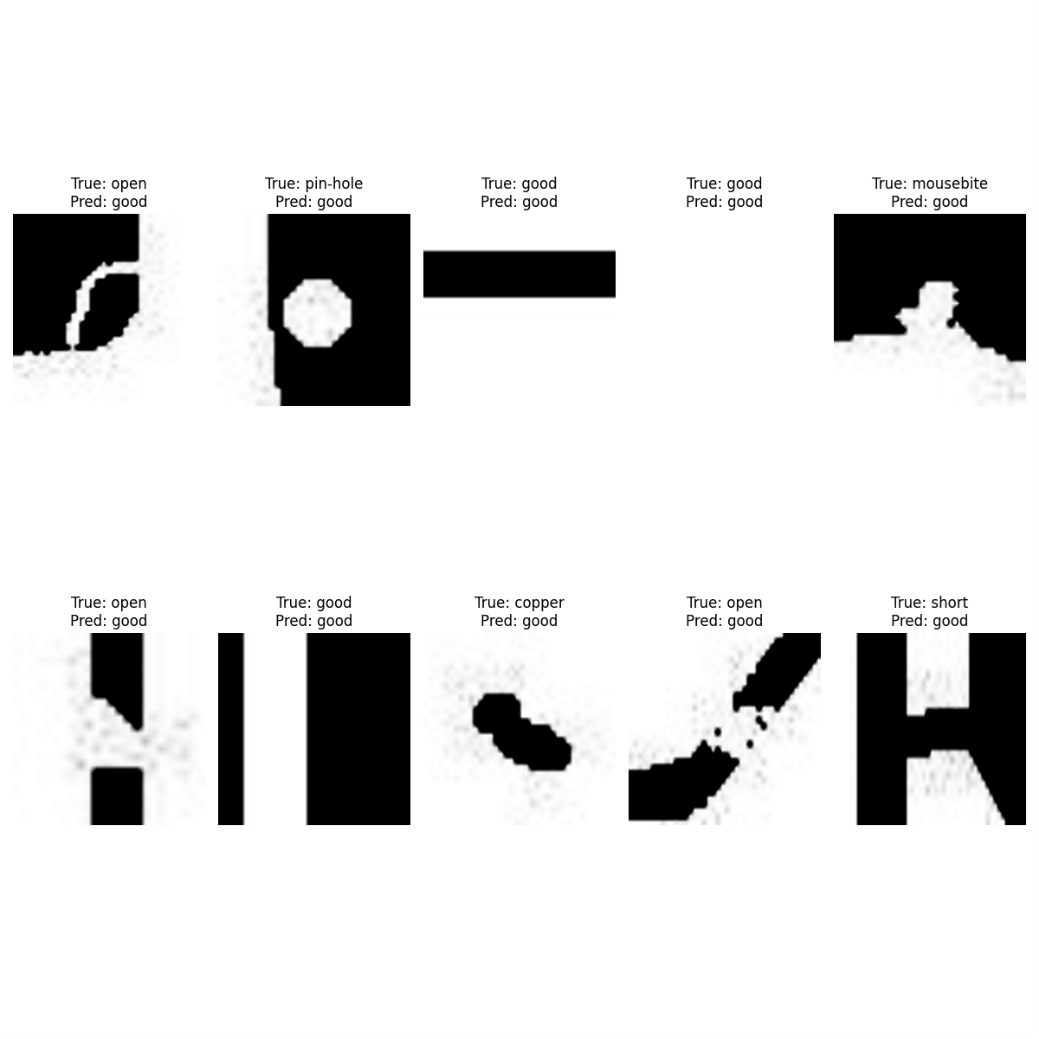
\includegraphics[width=0.35\textwidth]{./img/VGG/P7.png}
    \caption{VGG GAN 可視化結果} 
    \label{fig:VGG_P7}
\end{figure}
\begin{figure}[H]
    \centering
    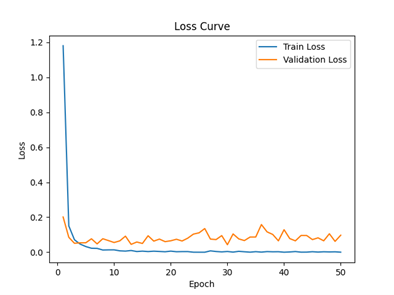
\includegraphics[width=0.45\textwidth]{./img/VGG/P8.png}
    \caption{VGG B8 Lr2e-5 GAN Loss曲線}
    \label{fig:VGG_P8}
\end{figure}
\begin{figure}[H]
    \centering
    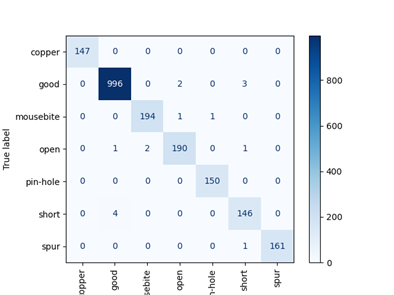
\includegraphics[width=0.45\textwidth]{./img/VGG/P9.png}
    \caption{VGG B8 Lr2e-5 GAN confusion matrix}
    \label{fig:VGG_P9}
\end{figure}
\begin{figure}[H]
    \centering
    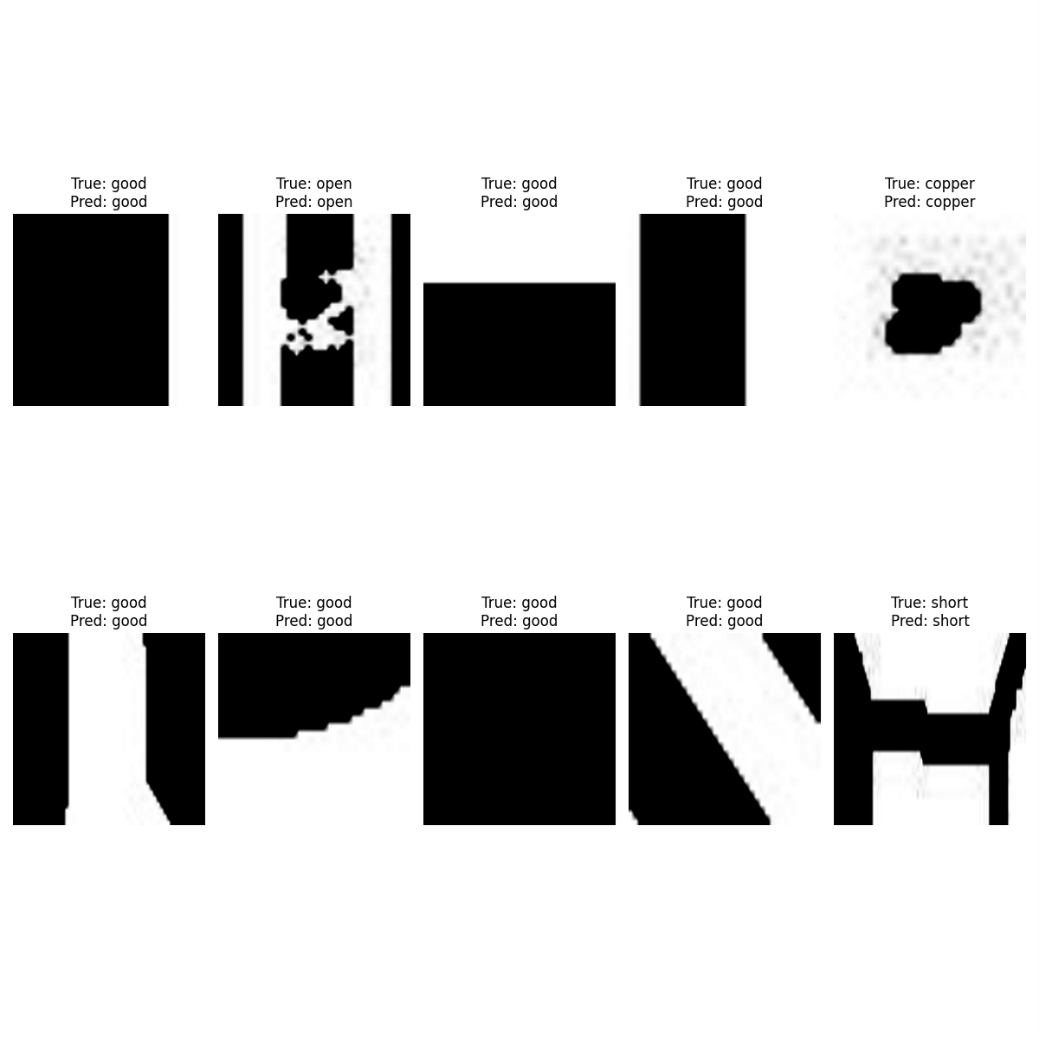
\includegraphics[width=0.35\textwidth]{./img/VGG/P10.png}
    \caption{VGG B8 Lr2e-5 GAN 可視化結果}
    \label{fig:VGG_P10}
\end{figure}
%

%   GoogLeNet
\begin{abstract}
    \noindent\textbf{C. GoogLeNet}\\
    %
    在GoogLeNet的模型訓練當中,觀察accurracy、loss曲線:
    \begin{enumerate}
        \item 隨著Batch size的減少,在Batch size 64時loss 會有很大的震盪,在Batch size 32時,震盪會收斂變小,而在Batch size 8 會呈現平滑。
        \item 準確率也隨Batch size減少而震盪減少,在Batch size 64會有很大的震盪。
        \item Train loss在epoch 10~20左右就會收斂。
    \end{enumerate}
    %
    在GoogLeNet的模型訓練當中,觀察confusion matrix與其指標:
    \begin{enumerate}
        \item 在Batch size 8和Batch size 32時,多數特徵會辨識為good。
        \item 承上點,若這種狀況發生時,瑕疵的precision會較高,而recall會較低,和瑕疵檢測所需要的高recall矛盾,所以應該避免此類參數。
    \end{enumerate}
    %
    加入GAN之後的變化:
    \begin{enumerate}
        \item 加入GAN之後,還是會有震盪,只是變成集中在Epochs 30以前,過Epoch 30 之後震盪明顯變小。
        \item Train Loss 收斂速度差不多。
    \end{enumerate}
\end{abstract}
%
\begin{figure}[H]
    \centering
    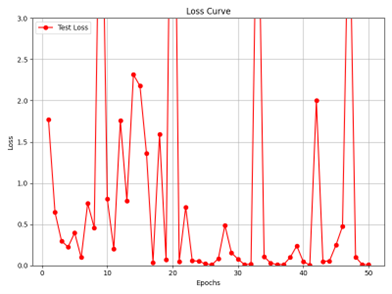
\includegraphics[width=0.40\textwidth]{./img/GoogLeNet/P1.png}
    \caption{GoogLeNet loss曲線}
    \label{fig:GoogLeNet_P1}
\end{figure}
\begin{figure}[H]
    \centering
    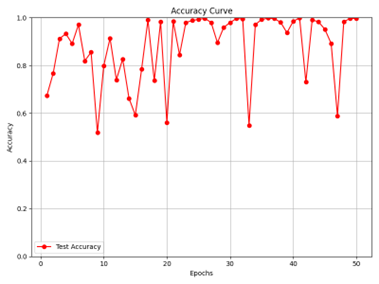
\includegraphics[width=0.40\textwidth]{./img/GoogLeNet/P2.png}
    \caption{GoogLeNet accuracy曲線}
    \label{fig:GoogLeNet_P2}
\end{figure}
%
\FloatBarrier

%   ResNet
\begin{abstract}
    \noindent\textbf{D. ResNet}\\
    在ResNet的模型訓練當中,觀察accurracy、loss曲線:
    \begin{enumerate}
        \item ResNet在訓練中不論是有無使用GAN擴充的資料集,近乎都是呈現無法收斂的情況\ref{fig:ResNet_unconvergence_loss_curve},除了設定batch size為32,learning rate為1e-4或2e-5的情況有收斂完成。
        \item 在準確度上也對應了loss曲線的情況,因未成功收斂而導致準確度較差,在特定數據下才有準確率達到0.97的情況\ref{fig:ResNet_accuracy_curve}。
        \item 針對有使用GAN的資料集,在loss曲線有收斂完成的情況下,準確率較無使用GAN的資料集略低0.01左右。
    \end{enumerate}
    在ResNet的模型訓練當中,觀察confusion matrix與其指標:
    \begin{enumerate}
        \item 對於同一個class,在loss曲線有收斂完成的情況下,precision與recall都達到0.96左右,而未完成收斂的情況則是precision明顯高於recall。
        \item 以confusion matrix綜觀全部的classes,最差的表現通常落在open、good,而以open的情況又較差\ref{fig:ResNet_confusion_matrix}。
    \end{enumerate}
\end{abstract}
%   ResNet Figure
\begin{figure}[H]
    \centering
    \includegraphics[width=0.45\textwidth]{./ResNet/runs/colorless_with_GAN/Fold2/train_e50_b64_lr0.001/train_valid_loss_curve.png}
    \caption{ResNet未收斂loss曲線}
    \label{fig:ResNet_unconvergence_loss_curve}
\end{figure}
\begin{figure}[H]
    \centering
    \includegraphics[width=0.45\textwidth]{./ResNet/runs/colorless_with_GAN/Fold2/train_e50_b32_lr0.0001/train_valid_loss_curve.png}
    \caption{ResNet已收斂loss曲線}
    \label{fig:ResNet_convergence_loss_curve}
\end{figure}
\begin{figure}[H]
    \centering
    \includegraphics[width=0.45\textwidth]{./ResNet/runs/colorless_with_GAN/Fold2/train_e50_b32_lr0.0001/train_valid_accuracy_curve.png}
    \caption{ResNet Accuracy曲線}
    \label{fig:ResNet_accuracy_curve}
\end{figure}
\begin{figure}[H]
    \centering
    \includegraphics[width=0.45\textwidth]{./ResNet/runs/colorless_with_GAN/Fold2/train_e50_b32_lr0.0001/confusion_matrix.png}
    \caption{ResNet Confusion Matrix}
    \label{fig:ResNet_confusion_matrix}
\end{figure}
%
\FloatBarrier

%   SqueezeNet
\begin{abstract}
    \noindent\textbf{E. SqueezeNet}\\
    在SqueezeNet的模型訓練當中,觀察accurracy、loss曲線:
    \begin{enumerate}
        \item SqueezeNet在不論是有無使用GAN進行擴充的資料集下,loss曲線幾乎都有收斂\ref{fig:SqueezeNet_convergence_loss_curve},除了在batch size為8與learning rate為1e-3,以本次實驗來說batch size極小learning rate極大的情況下,loss曲線完全沒有收斂\ref{fig:SqueezeNet_unconvergence_loss_curve},甚至是模型完全沒有學習到特徵。
        \item 而在learning rate為1e-3的情況下,多數的loss曲線會在epoch為10左右出現較大的起伏\ref{fig:SqueezeNet_unconvergence_loss_curve_1e-3},進而影響到後面的模型收斂與最後的準確率。
        \item 準確度上因為多數情況下loss曲線都有收斂,所以準確度普遍落在0.96左右\ref{fig:SqueezeNet_accuracy_curve_0.96},在learning rate為1e-3,並且最後有收斂的情況下,準確率在0.69左右\ref{fig:SqueezeNet_accuracy_curve_0.69}。
        \item 針對有使用GAN的資料集,在loss曲線有收斂完成的情況下,準確率與無使用GAN的資料集無明顯差異。
    \end{enumerate}
    在SqueezeNet的模型訓練當中,觀察confusion matrix與其指標:
    \begin{enumerate}
        \item 對於同一個class,在loss曲線有收斂完成的情況下,precision與recall都達到0.96左右,而未完成收斂的情況則是precision與recall數據持平,表示模型並沒有完整學習到特徵。
        \item 以confusion matrix綜觀全部的classes,最差的表現通常落在open、good,又以open的情況又較差\ref{fig:SqueezeNet_confuson_matrix}。
    \end{enumerate}
\end{abstract}
%   SqueezeNet Figure
\begin{figure}[H]
    \centering
    \includegraphics[width=0.40\textwidth]{./SqueezeNet/runs/colorless_with_GAN/Fold2/train_e50_b32_lr0.0001/train_valid_loss_curve.png}
    \caption{SqueezeNet已收斂loss曲線}
    \label{fig:SqueezeNet_convergence_loss_curve}
\end{figure}
\begin{figure}[H]
    \centering
    \includegraphics[width=0.40\textwidth]{./SqueezeNet/runs/colorless_with_GAN/Fold2/train_e50_b8_lr0.001/train_valid_loss_curve.png}
    \caption{SqueezeNet之loss曲線表示模型無學習到特徵}
    \label{fig:SqueezeNet_unconvergence_loss_curve}
\end{figure}
\begin{figure}[H]
    \centering
    \includegraphics[width=0.40\textwidth]{./SqueezeNet/runs/colorless_with_GAN/Fold2/train_e50_b32_lr0.001/train_valid_loss_curve.png}
    \caption{SqueezeNet之loss曲線收斂但較不穩}
    \label{fig:SqueezeNet_unconvergence_loss_curve_1e-3}
\end{figure}
\begin{figure}[H]
    \centering
    \includegraphics[width=0.40\textwidth]{./SqueezeNet/runs/colorless_with_GAN/Fold2/train_e50_b32_lr0.0001/train_valid_accuracy_curve.png}
    \caption{SqueezeNet Accuracy曲線}
    \label{fig:SqueezeNet_accuracy_curve_0.96}
\end{figure}
\begin{figure}[H]
    \centering
    \includegraphics[width=0.40\textwidth]{./SqueezeNet/runs/colorless_with_GAN/Fold2/train_e50_b32_lr0.001/train_valid_accuracy_curve.png}
    \caption{SqueezeNet Accuracy曲線}
    \label{fig:SqueezeNet_accuracy_curve_0.69}
\end{figure}
\begin{figure}[H]
    \centering
    \includegraphics[width=0.40\textwidth]{./SqueezeNet/runs/colorless_with_GAN/Fold2/train_e50_b32_lr0.0001/confusion_matrix.png}
    \caption{SqueezeNet Confusion Matrix}
    \label{fig:SqueezeNet_confuson_matrix}
\end{figure}
%

%   Xception
\begin{abstract}
    \noindent\textbf{F. Xception}
    \\Learning rate觀察:

    當batch size = 64,且learning rate為1e-3(圖\ref{fig:Xception_P1})、1e-4(圖\ref{fig:Xception_P2})時,valid loss會產生大幅波動,波動的頻率隨著learning rate的降低而趨緩;
    而valid loss在learning rate為2e-5(圖\ref{fig:Xception_P3})時,valid loss曲線恢復正常收斂。

    對於本資料集,較大的learning rate(1e-3、1e-4)可能導致模型參數修正過於劇烈,造成accuracy與loss曲線劇烈波動,
    而較小的learning rate(2e-5)有著最穩定accuracy與loss曲線。
    %
    \\Batch size觀察:

    當learning rate = 2e-5,且batch size為8(圖\ref{fig:Xception_P4})、32(圖\ref{fig:Xception_P5})時,valid loss會產生大幅波動,波動頻率隨著batch size的上升而趨緩;
    當batch size為64(圖\ref{fig:Xception_P3})時,valid loss曲線恢復正常收斂。

    對於本資料集,較小的batch size(8、32)可能導致模型參數修正過於劇烈,造成accuracy與loss曲線的劇烈波動,
    而較大的batch size(64)有著最穩定accuracy與loss曲線。
    %
    \\模型總結:

    較小的Learning rate與較大的Batch size更適合本資料集,可以得到更加穩定的訓練過程。
\end{abstract}
%
\begin{figure}[H]
    \centering
    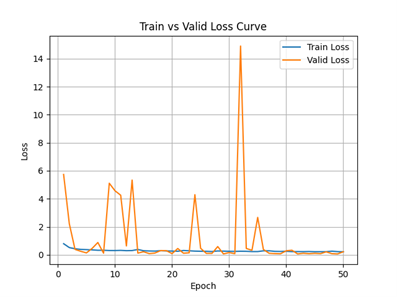
\includegraphics[width=0.40\textwidth]{./img/Xception/P1.png}
    \caption{Xception B64 Lr1e-3 Loss曲線}
    \label{fig:Xception_P1}
\end{figure}
\begin{figure}[H]
    \centering
    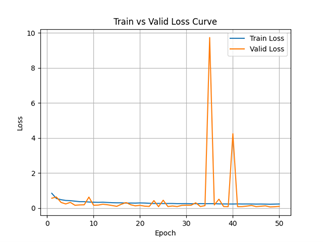
\includegraphics[width=0.40\textwidth]{./img/Xception/P2.png}
    \caption{Xception B64 Lr1e-4 Loss曲線}
    \label{fig:Xception_P2}
\end{figure}
\begin{figure}[H]
    \centering
    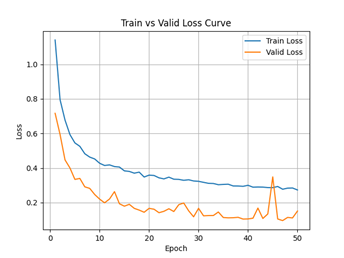
\includegraphics[width=0.40\textwidth]{./img/Xception/P3.png}
    \caption{Xception B64 Lr2e-5 Loss曲線}
    \label{fig:Xception_P3}
\end{figure}
\begin{figure}[H]
    \centering
    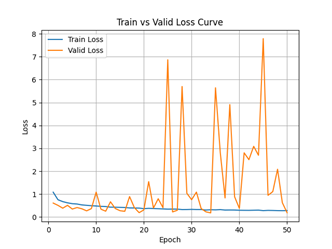
\includegraphics[width=0.40\textwidth]{./img/Xception/P4.png}
    \caption{Xception B8 Lr2e-5 Loss曲線}
    \label{fig:Xception_P4}
\end{figure}
\begin{figure}[H]
    \centering
    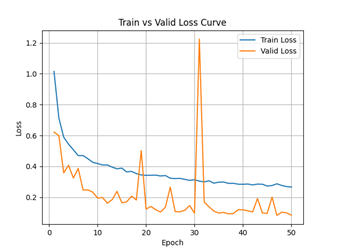
\includegraphics[width=0.40\textwidth]{./img/Xception/P5.png}
    \caption{Xception B32 Lr2e-5 Loss曲線}
    \label{fig:Xception_P5}
\end{figure}
%
\FloatBarrier

%   MobileNetV1
\begin{abstract}
    \noindent\textbf{G. MobileNetV1}\\
    在MoblieNetV1的模型訓練當中,觀察accurracy、loss曲線:
    \begin{enumerate}
        \item Loss約在epoch30左右收斂。
        \item 但當learning rate增加(約1e-4,1e-3),會震盪且無發收斂;Batch size 減少也會有一樣情況,但主要依learning 為主。
        \item 此模在此次實驗數據中,以較高的batch size 和 較小的learning rate 表現較好。
    \end{enumerate}
    %
    在MoblieNet的模型訓練當中,觀察confusion matrix與其指標:
    \begin{enumerate}
        \item 在learning rate 1e-3時,部分模型將good預測為其他特徵,如mousebite、spur等等。
    \end{enumerate}
    %
    加入GAN之後的變化:
    \begin{enumerate}
        \item 在加入GAN後,平均精度(mAP)有些微上升約1~2\%。
    \end{enumerate}
\end{abstract}
%

%   MNASNet
\begin{abstract}
    \noindent\textbf{H. MNASNet}\\
    \hspace*{2em}在MNASNet的訓練結果中,我們可以發現,訓練的valid loss基本上都沒有收斂,
    形狀為跳動(圖\ref{fig:MNASNet_P1})或呈現V形(圖\ref{fig:MNASNet_P2}),且結果十分不穩定,接下來透過分析confusion matrix中的結果來推導原因。
    %
    batch size為8的情況:
    \begin{enumerate}[1.]
        \item learning rate為1e-3時,原始資料只有在fold 1的epoch 30有呈現正常辨識結果,剩餘的皆集中判定成一到三個特徵,
              其中最容易將各特徵判定為good,(圖\ref{fig:MNASNet_P3})。
              增加GAN生成的資料集,在epoch 50時,都有較為準確的辨識,但仍可看出部分good被辨識為瑕疵或是瑕疵被辨識為good(圖\ref{fig:MNASNet_P4}為部分good被辨識為瑕疵,圖\ref{fig:MNASNet_P5}為部分瑕疵被辨識為good),
              而epoch 10及30時,有時會將大部分特徵辨識為good,有時能正常辨識各特徵,且辨識效果不一定比epoch 50還要差。
        \item Learning rate為1e-4與2e-5時,epoch 10的訓練結果全都會辨識成good(圖\ref{fig:MNASNet_P6}),而在epoch 30時,大都有辨識正確,
              部份good被辨識為瑕疵或是瑕疵被辨識為good,epoch 50與epoch 30的結果相似,不一定較為準確,但會出現極端狀況,像是good全部都辨識為good,但瑕疵部份辨識正確,部份被辨識為good(圖\ref{fig:MNASNet_P7})。
    \end{enumerate}
    %
    batch size為32的情況:
    \begin{enumerate}[1.]
        \item 且learning rate為1e-3時,原資料集的epoch 10會將所有特徵辨識為good,epoch 30及50時,
              原資料集與增加GAN生成的資料集,會集中將各特徵辨識成某一特徵,此特徵為good的頻率最高(7/12),
              open次之(3/12),最後是spur(1/12),唯一一次正常辨識的是增加GAN生成的資料集的fold 3 epoch 50(1/12),另外,雖然集中辨識為某一特徵,仍可發現極小部分的特徵被正確辨識。
        \item learning rate為1e-4時,原資料集各epoch結果,幾乎是將所有特徵辨識為good,但增加GAN生成的資料集,在epoch 50時,可以較明顯的看出正確辨識結果,但仍有大量good被辨識為瑕疵或是瑕疵被辨識為good。
        \item learning rate為2e-5時,不論有無增加GAN生成圖片,各特徵皆被辨識為good。
    \end{enumerate}
    %
    Batch size 為64的情況:
    \begin{enumerate}[1.]
        \item learning rate為1e-3時,在原資料集與增加GAN生成的資料集的epoch 10與epoch 30中,
              特徵皆被全數辨識為good。而epoch 50時,原資料集在fold 1中較能辨識各特徵但仍有大量good被辨識為瑕疵或是瑕疵被辨識為good的情況,
              剩餘兩個fold中,各特徵幾乎被辨識為good,增加GAN生成的資料集,會各特徵特定辨識成某幾個固定特徵,或是呈現不規則的分布。
        \item learning rate為1e-4與2e-5時,各特徵皆被辨識為good。
    \end{enumerate}
    %
    分析Precision與Recall的數據:
    \begin{enumerate}[1.]
        \item 若是全數被辨識為good,原資料集的Precision會是0.0715,增加GAN生成圖片的資料集的Precision會是0.0662,而兩者Recall皆為0.1429。
        \item 第一點的情況,在batch size越大及learning rate越小的時候,越容易發生。
        \item 其餘的數據非常不穩定,例如在batch size為8,learning rate為1e-3的時候,原資料集三個fold的Precision分別為0.9105、0.256、0.6202。三者相差甚遠,
              可以看出相同的參數下,結果的優劣各有不同。同樣的參數,在fold2中epoch 10到50的precision分別為0.014、0.9341、0.256,
              同樣非常不穩定,另外同時觀測loss curve(跳動形狀)可以發現,0.9341恰好是出現在valid loss中相對較低的點。
    \end{enumerate}
    %
    結論推導:
    \begin{enumerate}[1.]
        \item 各參數的valid loss皆無法收斂,而跳動的valid loss,其低點有可能產生出較好的實驗結果。
        \item 訓練結果中很容易出現全數被辨識為特定特徵的情況,其中又以全數被辨識為good最為頻繁出現。
        \item 某些參數是能較為正常辨識特徵的,但仍有good被辨識為瑕疵或是瑕疵被辨識為good。
        \item 在Batch size較大的情況下,越小的learning rate,越容易將各特徵全數辨識為good。
        \item epoch為10時,時常會出現將所有特徵全數辨識為good的情況。
    \end{enumerate}
    模型總結:
    \begin{enumerate}[1.]
        \item 在此實驗中,時常出現全數辨識為good,以及good被辨識為瑕疵或是瑕疵被辨識為good的情況。
              而good這個特徵又恰好是兩個資料集中圖片總數最多的一個特徵,因而造成了模型較易將各特徵辨識為good,或是較明顯的將good誤檢的的情況。
        \item 在此資料集中,MNASNet不適合較大的batch size以及較小的learning rate同時出現。
    \end{enumerate}
\end{abstract}
%
\begin{figure}[H]
    \centering
    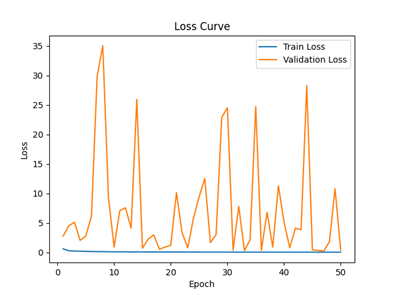
\includegraphics[width=0.45\textwidth]{./img/MNASNet/P1.png}
    \caption{MNASNet 跳動 Loss曲線}
    \label{fig:MNASNet_P1}
\end{figure}
\begin{figure}[H]
    \centering
    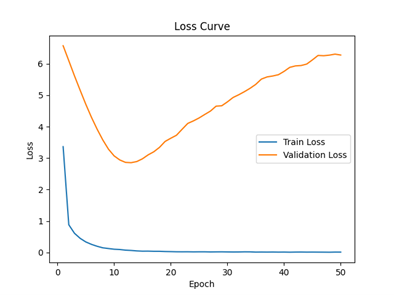
\includegraphics[width=0.45\textwidth]{./img/MNASNet/P2.png}
    \caption{MNASNet V型 Loss曲線}
    \label{fig:MNASNet_P2}
\end{figure}
\begin{figure}[H]
    \centering
    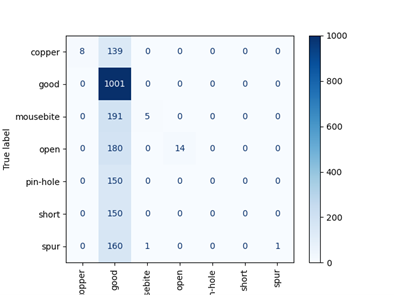
\includegraphics[width=0.45\textwidth]{./img/MNASNet/P3.png}
    \caption{MNASNet 集中辨識為good\protect\\
    confusion matrix}
    \label{fig:MNASNet_P3}
\end{figure}
\begin{figure}[H]
    \centering
    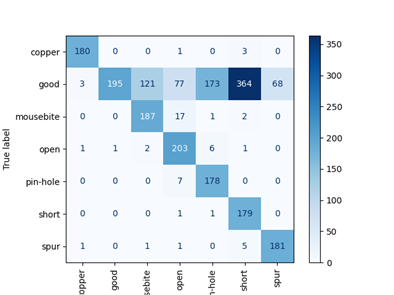
\includegraphics[width=0.45\textwidth]{./img/MNASNet/P4.png}
    \caption{MNASNet 部分good辨識為瑕疵\protect\\
             confusion matrix}
    \label{fig:MNASNet_P4}
\end{figure}
\begin{figure}[H]
    \centering
    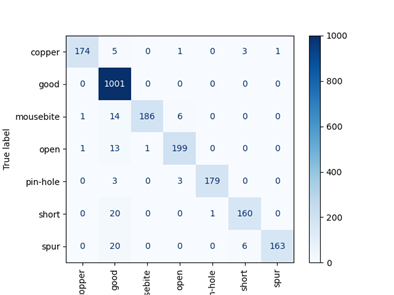
\includegraphics[width=0.45\textwidth]{./img/MNASNet/P5.png}
    \caption{MNASNet 部分瑕疵辨識為good\protect\\
             confusion matrix}
    \label{fig:MNASNet_P5}
\end{figure}
\begin{figure}[H]
    \centering
    \includegraphics[width=0.45\textwidth]{./img/MNASNet/P6.png}
    \caption{MNASNet 全瑕疵辨識為good\protect\\
             confusion matrix}
    \label{fig:MNASNet_P6}
\end{figure}
\begin{figure}[H]
    \centering
    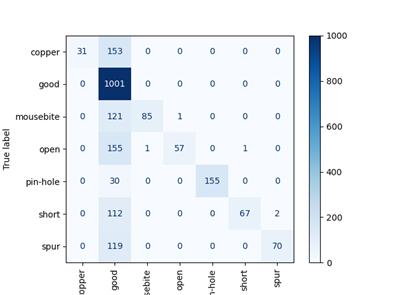
\includegraphics[width=0.45\textwidth]{./img/MNASNet/P7.png}
    \caption{MNASNet good正確辨識、\protect\\
             部分瑕疵辨識為good confusion matrix}
    \label{fig:MNASNet_P7}
\end{figure}
%
\FloatBarrier

%EfficientNet
\begin{abstract}
    \noindent\textbf{I. EfficientNet}\\
    EfficientNet原始資料集訓練結果中
    \begin{enumerate}
        \item Epoch值較大時,模型訓練表現Loss確實略微下降。注意到隨著Batch size值較大時,Loss下降較為明顯。
        \item 觀察到隨著Batch size值越大,訓練表現的Loss略為增加。
    \end{enumerate}
    %
    GAN生成資料集的表現特點
    \begin{enumerate}
        \item 表現與原始資料集相比,並無明顯差別。
        \item 觀察相同Epoch= 50與 Learning Rate= 2e-5的條件下,Batch Size的增加Loss的表現無明顯改善。
    \end{enumerate}
\end{abstract}
%
\begin{figure}[H]
    \centering
    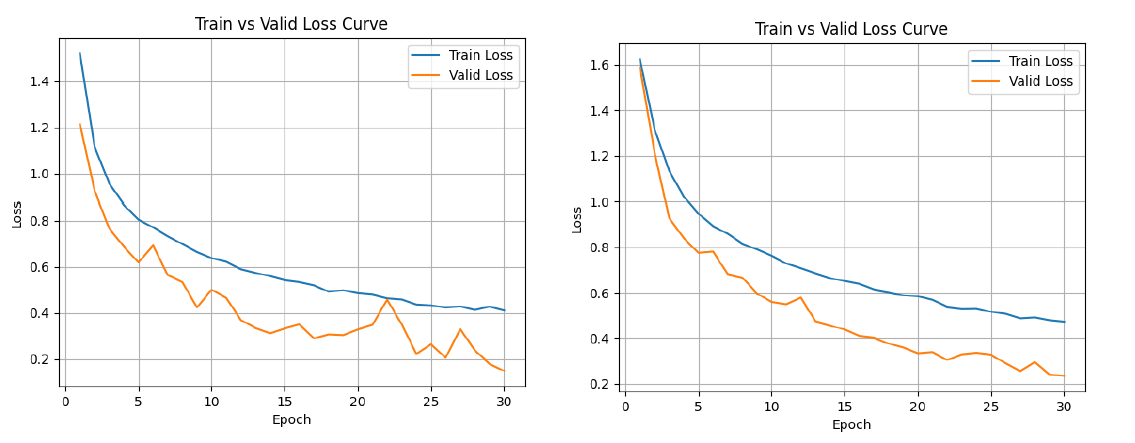
\includegraphics[width=0.45\textwidth]{./img/EfficientNet/P1.png}
    \caption{EfficientNet epoch30 Lr2e-5 Loss曲線\protect\\(左:Batch size32,右:Batch size64)}
    \label{fig:EfficientNet_P1}
\end{figure}
\begin{figure}[H]
    \centering
    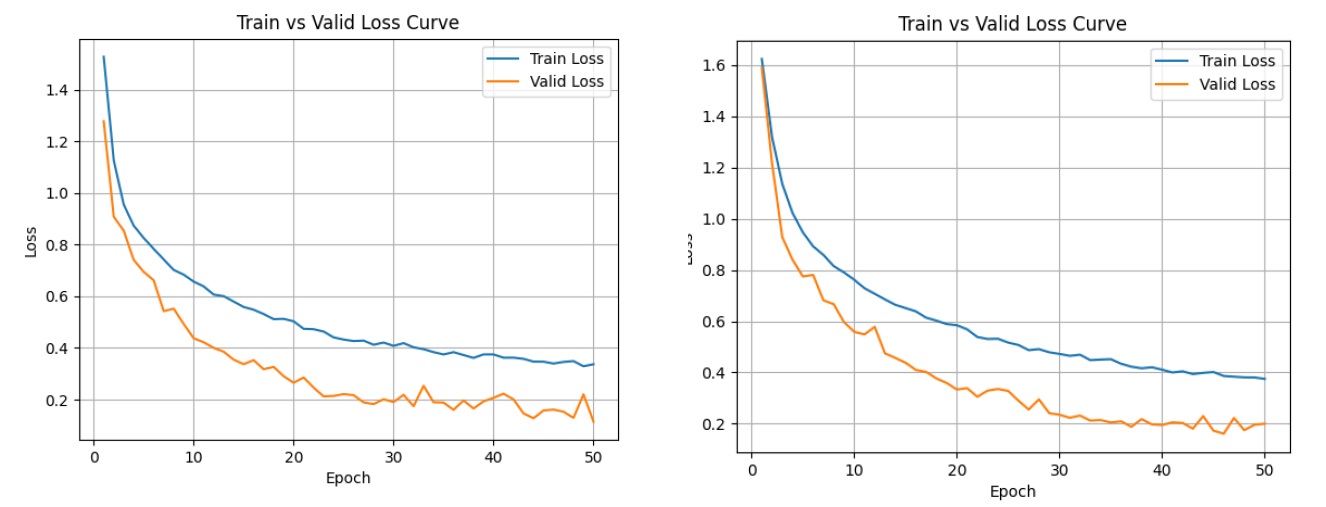
\includegraphics[width=0.45\textwidth]{./img/EfficientNet/P2.png}
    \caption{EfficientNet epoch50 Lr2e-5 Loss曲線\protect\\(左:Batch size32,右:Batch size64)}
    \label{fig:EfficientNet_P2}
\end{figure}
\begin{figure}[H]
    \centering
    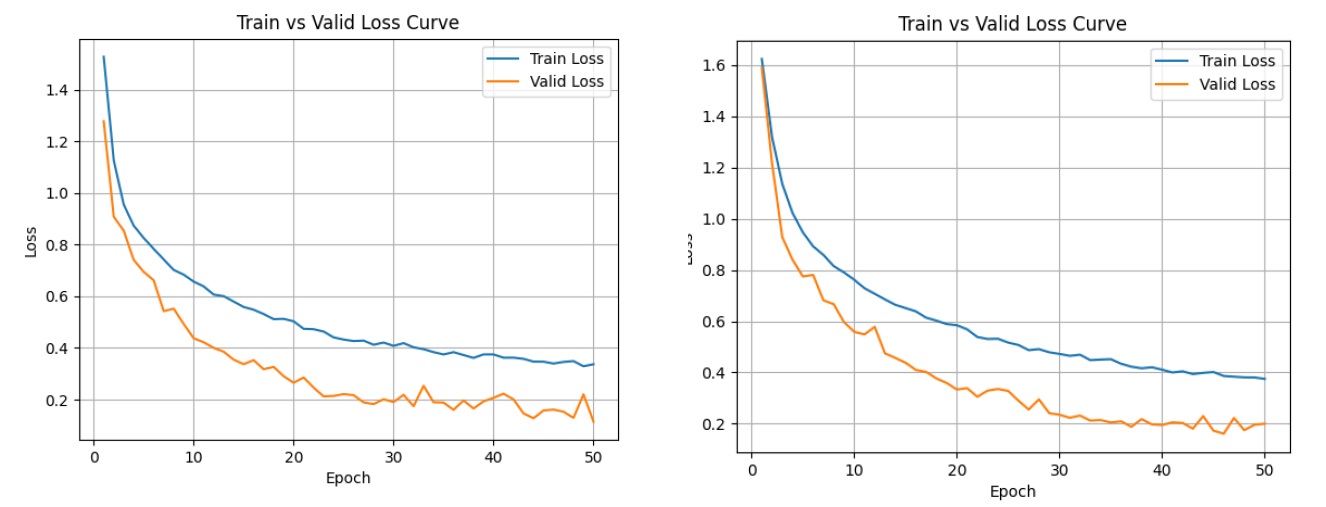
\includegraphics[width=0.45\textwidth]{./img/EfficientNet/P2.png}
    \caption{EfficientNet epoch50 Lr2e-5 GAN Loss曲線\protect\\(左:Batch size32,右:Batch size64)}
    \label{fig:EfficientNet_P3}
\end{figure}
%
\FloatBarrier

%   ViT
\begin{abstract}
    \noindent\textbf{K. ViT}\\
    在ViT的模型訓練當中,觀察accurracy、loss曲線:
    \begin{enumerate}
        \item 隨著learning rate增加,模型收斂的速度也隨之增快,若learning rate過低(如lr = 1e-3),會有可能遇到模型收斂困難的問題。
        \item 模型訓練的準確度在epoch10~20的區間時就已經接近100\%,訓練集準確度接近100\%,但驗證集的準確率在收斂至約95\%時就不再收斂。
        \item 更改batch size參數,batch size提升時整體loss皆有下降的趨勢,準確率也有相對提升,不過隨著learning rate提升,改變batch size所造成的影響也隨之變小。
    \end{enumerate}
    %
    在ViT的模型訓練當中,觀察confusion matrix與其指標:
    \begin{enumerate}
        \item 對於同一個class,有時候Precision會低於Recall,有時Precision高於Recall,表示模型漏檢或是誤報的現象並不固定。
        \item 綜觀全部的class,表現最差class大多都落在open、short、spur,而open的表現最差,約落在90\%。
    \end{enumerate}
    %
    加入GAN之後的變化:
    \begin{enumerate}
        \item 對於整個訓練來說,隨著epoch增加的模型收斂速度有略為提升。
        \item 在較低learning rate當中的表現有得到不錯的提升,到了lr=2e-5原本就很高的準確率也上升了1~2\%。
    \end{enumerate}
\end{abstract}
%
\begin{figure}[H]
    \centering 
    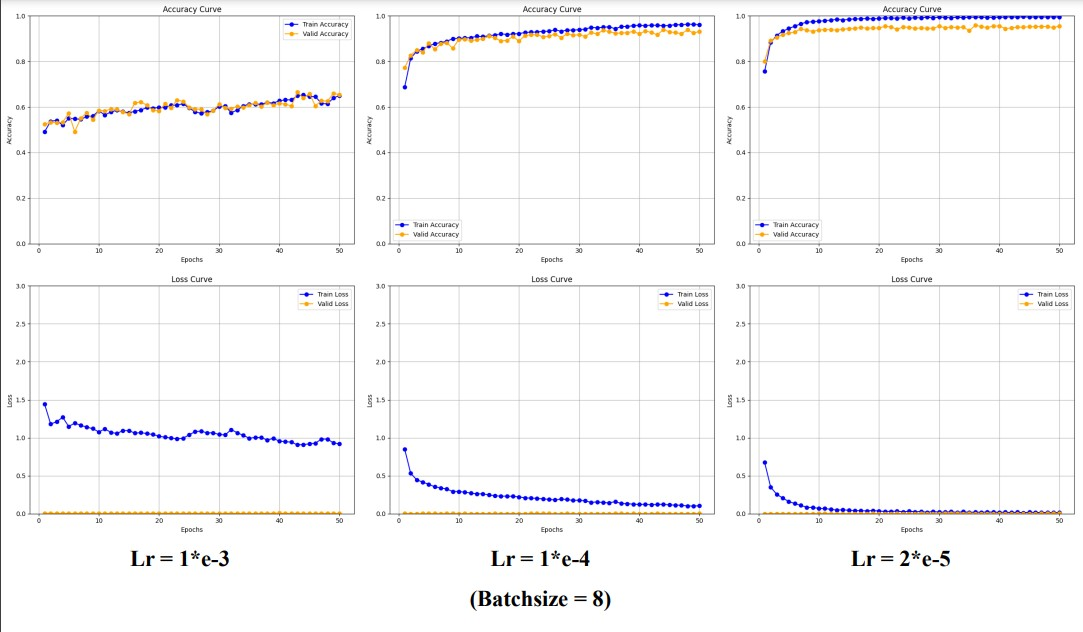
\includegraphics[width=0.85\linewidth, height=4cm]{img/ViT_b8.jpg} 
    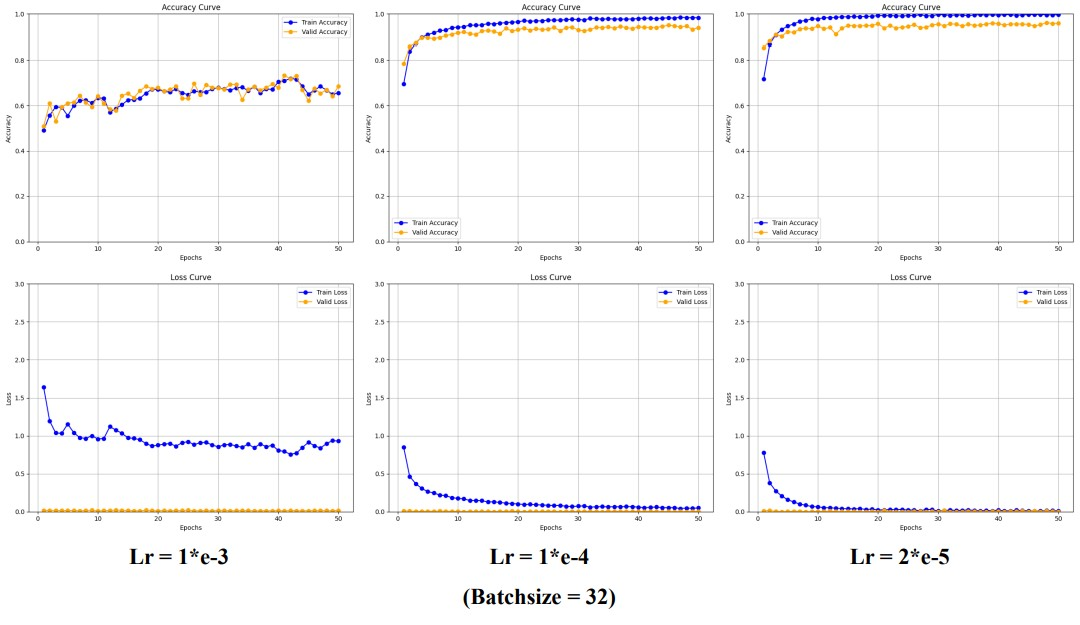
\includegraphics[width=0.85\linewidth, height=4cm]{img/ViT_b32.jpg}
    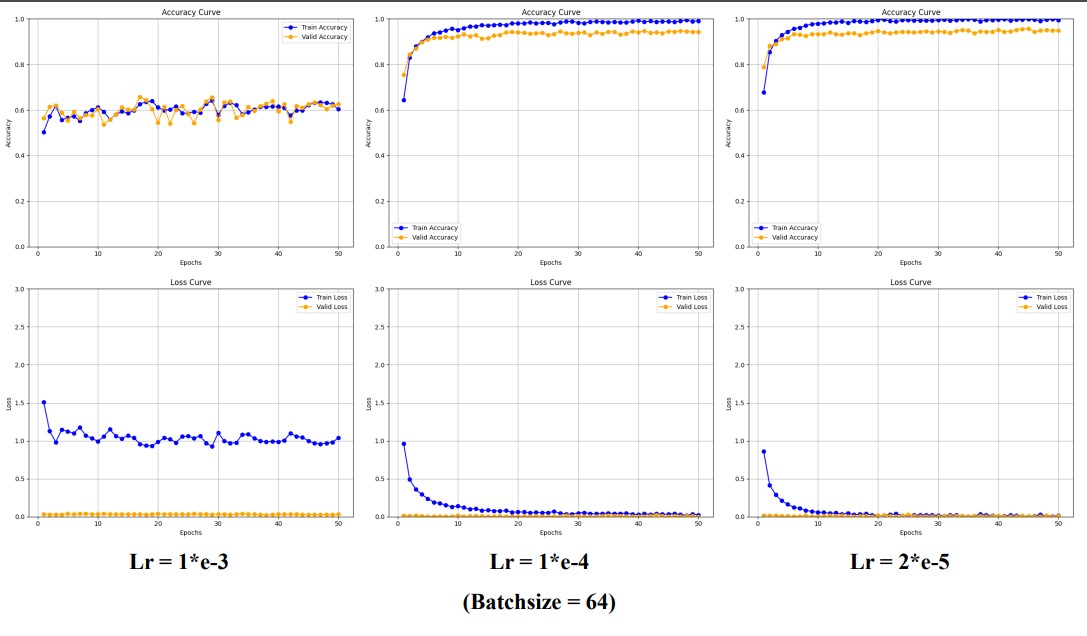
\includegraphics[width=0.85\linewidth, height=4cm]{img/ViT_b64.jpg}
    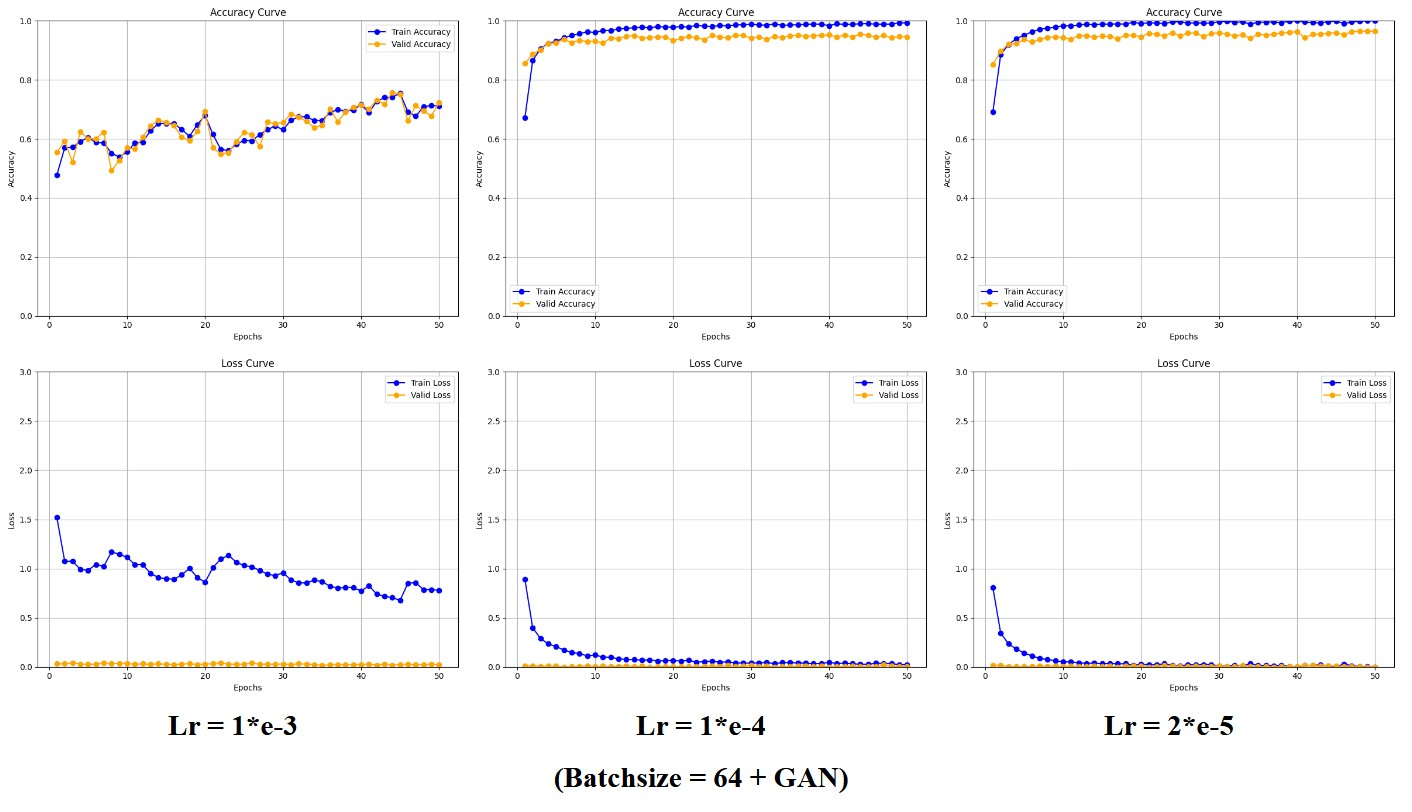
\includegraphics[width=0.85\linewidth, height=4cm]{img/ViT_b64_GAN.jpg}
    \caption{ViT訓練結果}
\end{figure}
%

%   ConvNeXt
\begin{abstract}
    \noindent\textbf{L. ConvNeXt}
    \\Learning rate觀察:
    
    此模型於相同batch Size時,在learning rate為1e-3時,20個epoch內便能使valid loss低於0.2(圖\ref{fig:ConvNeXt_P1}),30個epoch的valid accuracy已達0.95(圖\ref{fig:ConvNeXt_P2});
    在learning rate為2e-5時,50個epoch的valid loss卻依然高於0.3(圖\ref{fig:ConvNeXt_P3}),且valid accuracy只到達0.9(圖\ref{fig:ConvNeXt_P4})。
    
    對於PCB瑕疵資料集,較大的learning rate(1e-3)有著最快的收斂速度及最高的test accuracy。
    %
    \\Batch size觀察:

    此模型於相同learning rate時,batch size為8與64的loss curve(圖\ref{fig:ConvNeXt_P5})與accuracy curve(圖\ref{fig:ConvNeXt_P6})極其相似,且test result(表\ref{table:ConvNeXt_T2})的各項數值差距均於10\%以內。

    當batch size由8提升至64時,recall與F1 score皆略微提升,precision略微降低。Batch size為32時,mPA、TestLoss和TestAccuracy有著最佳表現,有著最低的loss與最高的accuracy。
    %
    \\模型總結:
    \begin{enumerate}
        \item 對本資料集較大的Learning rate(1e-3)更適合,有著更快的收斂速度及更高的準確率。
        \item 對本資料集Batch size為32最適合,可於最多的指標獲得最佳效果。
    \end{enumerate}
\end{abstract}
%
\begin{figure}[H]
    \centering
    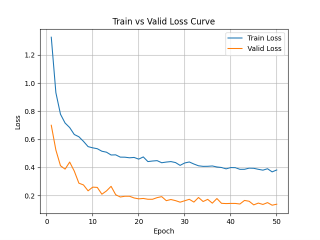
\includegraphics[width=0.45\textwidth]{./img/ConvNeXt/P1.png}
    \caption{ConvNeXt B64 Lr1e-3 Loss曲線}
    \label{fig:ConvNeXt_P1}
\end{figure}
\begin{figure}[H]
    \centering
    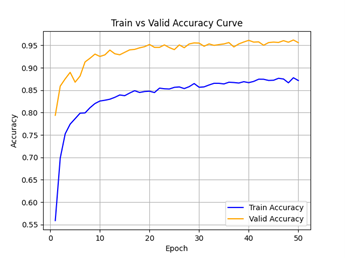
\includegraphics[width=0.45\textwidth]{./img/ConvNeXt/P2.png}
    \caption{ConvNeXt B64 Lr1e-3 Accuracy曲線}
    \label{fig:ConvNeXt_P2}
\end{figure}
\begin{figure}[H]
    \centering
    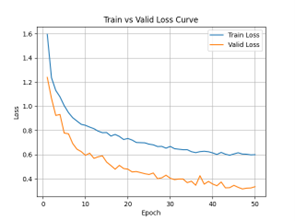
\includegraphics[width=0.45\textwidth]{./img/ConvNeXt/P3.png}
    \caption{ConvNeXt B64 Lr2e-5 Loss曲線}
    \label{fig:ConvNeXt_P3}
\end{figure}
\begin{figure}[H]
    \centering
    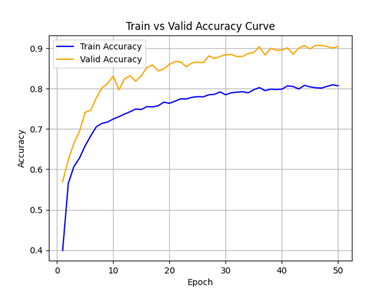
\includegraphics[width=0.45\textwidth]{./img/ConvNeXt/P4.png}
    \caption{ConvNeXt B64 Lr2e-5 Accuracy曲線}
    \label{fig:ConvNeXt_P4}
\end{figure}
\begin{table}[H]
    \footnotesize
    \centering
    \caption{ConvNeXt Batch size64 Test Result}
    \begin{tabular}{|r|c|c|c|c|c|c|c|c|}
        \hline
        & Precision & Recall & F1 Score & mAP & Loss & Accuracy \\
        \hline
        Lr1e-3 & 0.9512 & 0.946 & 0.9481 & 0.946 & 0.1335 & 0.9598 \\
        \hline
        Lr1e-4 & 0.9515 & 0.9247 & 0.9371 & 0.9247 & 0.1581 & 0.9571 \\
        \hline
        Lr1e-5 & 0.9002 & 0.876 & 0.8858 & 0.9876 & 0.2961 & 0.919 \\
        \hline
    \end{tabular}
    \label{table:ConvNeXt_T1}
\end{table}
\begin{figure}[H]
    \centering
    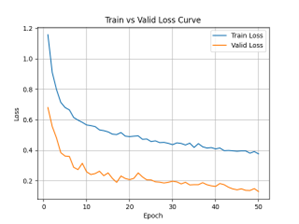
\includegraphics[width=0.45\textwidth]{./img/ConvNeXt/P5.png}
    \caption{ConvNeXt B8 Lr1e-3 Loss曲線}
    \label{fig:ConvNeXt_P5}
\end{figure}
\begin{figure}[H]
    \centering
    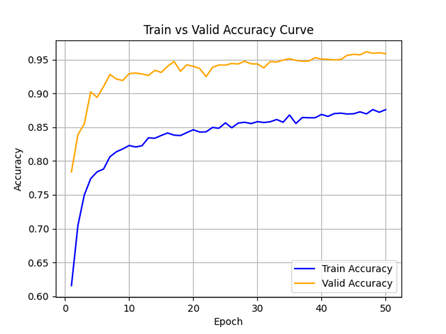
\includegraphics[width=0.45\textwidth]{./img/ConvNeXt/P6.png}
    \caption{ConvNeXt B8 Lr1e-3 Accuracy曲線}
    \label{fig:ConvNeXt_P6}
\end{figure}
\begin{table}[H]
    \footnotesize
    \centering
    \caption{ConvNeXt Learning rate1e-3 Test Result}
    \begin{tabular}{|r|c|c|c|c|c|c|c|}
        \hline
        & Precision & Recall & F1 Score & mAP & Loss & Accuracy \\
        \hline
        B8 & 0.9609 & 0.936 & 0.9474 & 0.936 & 0.1398 & 0.9598 \\
        \hline
        B32 & 0.9617 & 0.944 & 0.9523 & 0.944 & 0.1278 & 0.9633 \\
        \hline
        B64 & 0.9512 & 0.946 & 0.9481 & 0.946 & 0.1335 & 0.9598 \\
        \hline
    \end{tabular}
    \label{table:ConvNeXt_T2}
\end{table}
\FloatBarrier